
% Copyright (C) 2014-2016 by Thomas Auzinger <thomas@auzinger.name>

\documentclass[draft,final]{vutinfth} % Remove option 'final' to obtain debug information.

% Load packages to allow in- and output of non-ASCII characters.
\usepackage{lmodern}        % Use an extension of the original Computer Modern font to minimize the use of bitmapped letters.
\usepackage[T1]{fontenc}    % Determines font encoding of the output. Font packages have to be included before this line.
\usepackage[utf8]{inputenc} % Determines encoding of the input. All input files have to use UTF8 encoding.

% Extended LaTeX functionality is enables by including packages with \usepackage{...}.
\usepackage{fixltx2e}   % Provides fixes for several errors in LaTeX2e.
\usepackage{amsmath}    % Extended typesetting of mathematical expression.
\usepackage{amssymb}    % Provides a multitude of mathematical symbols.
\usepackage{mathtools}  % Further extensions of mathematical typesetting.
\usepackage{microtype}  % Small-scale typographic enhancements.
\usepackage{enumitem}   % User control over the layout of lists (itemize, enumerate, description).
\usepackage{multirow}   % Allows table elements to span several rows.
\usepackage{booktabs}   % Improves the typesettings of tables.
\usepackage{subcaption} % Allows the use of subfigures and enables their referencing.
\usepackage[ruled,linesnumbered,algochapter]{algorithm2e} % Enables the writing of pseudo code.
\usepackage[usenames,dvipsnames,table]{xcolor} % Allows the definition and use of colors. This package has to be included before tikz.
\usepackage{nag}       % Issues warnings when best practices in writing LaTeX documents are violated.
\usepackage{hyperref}  % Enables cross linking in the electronic document version. This package has to be included second to last.
\usepackage[acronym,toc]{glossaries} % Enables the generation of glossaries and lists fo acronyms. This package has to be included last.

% Define convenience functions to use the author name and the thesis title in the PDF document properties.
\newcommand{\authorname}{Matthias Plasser} % The author name without titles.
\newcommand{\thesistitle}{Title of the Thesis} % The title of the thesis. The English version should be used, if it exists.
% mycommands
\newcommand{\norm}[1]{\left\lVert#1\right\rVert}

% Set PDF document properties
\hypersetup{
    pdfpagelayout   = TwoPageRight,           % How the document is shown in PDF viewers (optional).
    linkbordercolor = {Melon},                % The color of the borders of boxes around crosslinks (optional).
    pdfauthor       = {\authorname},          % The author's name in the document properties (optional).
    pdftitle        = {\thesistitle},         % The document's title in the document properties (optional).
    pdfsubject      = {Subject},              % The document's subject in the document properties (optional).
    pdfkeywords     = {a, list, of, keywords} % The document's keywords in the document properties (optional).
}

\setsecnumdepth{subsection} % Enumerate subsections.

\nonzeroparskip             % Create space between paragraphs (optional).
\setlength{\parindent}{0pt} % Remove paragraph identation (optional).

\makeindex      % Use an optional index.
\makeglossaries % Use an optional glossary.
%\glstocfalse   % Remove the glossaries from the table of contents.

% Set persons with 4 arguments:
%  {title before name}{name}{title after name}{gender}
%  where both titles are optional (i.e. can be given as empty brackets {}).
\setauthor{}{\authorname}{}{male}
\setadvisor{Ao.univ.Prof. Dr.}{Andreas Rauber}{}{male}

% For bachelor and master theses:
\setfirstassistant{Pretitle}{Forename Surname}{Posttitle}{male}
\setsecondassistant{Pretitle}{Forename Surname}{Posttitle}{male}
\setthirdassistant{Pretitle}{Forename Surname}{Posttitle}{male}

% For dissertations:
\setfirstreviewer{Pretitle}{Forename Surname}{Posttitle}{male}
\setsecondreviewer{Pretitle}{Forename Surname}{Posttitle}{male}

% For dissertations at the PhD School:
\setsecondadvisor{Pretitle}{Forename Surname}{Posttitle}{male}

% Required data.
\setaddress{Address}
\setregnumber{0123456}
\setdate{01}{01}{2001} % Set date with 3 arguments: {day}{month}{year}.
\settitle{\thesistitle}{Effect of adversarial training on the decision boundary of convolutional neural networks} % Sets English and German version of the title (both can be English or German).
\setsubtitle{Optional Subtitle of the Thesis}{Optionaler Untertitel der Arbeit} % Sets English and German version of the subtitle (both can be English or German).

% Select the thesis type: bachelor / master / doctor / phd-school.
% Bachelor:
\setthesis{bachelor}
%
% Master:
%\setthesis{master}
%\setmasterdegree{dipl.} % dipl. / rer.nat. / rer.soc.oec. / master
%
% Doctor:
%\setthesis{doctor}
%\setdoctordegree{rer.soc.oec.}% rer.nat. / techn. / rer.soc.oec.
%
% Doctor at the PhD School
%\setthesis{phd-school} % Deactivate non-English title pages (see below)

% For bachelor and master:
\setcurriculum{Software and Information Engineering}{Software und Information Engineering} % Sets the English and German name of the curriculum.

% For dissertations at the PhD School:
\setfirstreviewerdata{Affiliation, Country}
\setsecondreviewerdata{Affiliation, Country}

% Define convenience macros.
\newcommand{\todo}[1]{{\color{red}\textbf{TODO: {#1}}}} % Comment for the final version, to raise errors.


\begin{document}

\frontmatter % Switches to roman numbering.
% The structure of the thesis has to conform to
%  http://www.informatik.tuwien.ac.at/dekanat

\addtitlepage{naustrian} % German title page (not for dissertations at the PhD School).
\addtitlepage{english} % English title page.
\addstatementpage

\begin{danksagung*}
\todo{Ihr Text hier.}
\end{danksagung*}

\begin{acknowledgements*}
\todo{Enter your text here.}
\end{acknowledgements*}

\begin{kurzfassung}
\todo{Ihr Text hier.}
\end{kurzfassung}

\begin{abstract}
\todo{Enter your text here.}
\end{abstract}

% Select the language of the thesis, e.g., english or naustrian.
\selectlanguage{english}

% Add a table of contents (toc).
\tableofcontents % Starred version, i.e., \tableofcontents*, removes the self-entry.

% Switch to arabic numbering and start the enumeration of chapters in the table of content.
\mainmatter

\chapter{Introduction}
Neural Networks are more reliable than ever in 2019, and outperform human experts in a broad range of tasks, from playing Go to recognizing fractures in MRIs. The existence of adversary examples - 
examples that are carefully, (almost) imperceptibly manipulated in order to get misclassified by neural networks challenges that reliability. Adversary inputs can be constructed by starting from
and input that is initially correctly labelled by a classifier. By carefully manipulating features by a tiny amount in the correct direction - towards the decision boundary, it's possible to
craft data that to a human still appears like the original input, yet gets labeled as something else by the given classifier. Adversarial inputs can even be crafted in hardware, like street signs. By adding special stickers, that do not influence a human's recognition, neural networks can be tricked to misclassify a picture of the manipulated sign. As long as neural networks can be fooled so easily, autonomous driving is very vulnerable.
A remedy against adversarial inputs is adversarial training - using those manipulated inputs for training.
In this paper, the effectiveness of different kinds of adversarial training, and especially how it influences the decision parameters of CNNs will be discussed and visualized. As decision parameters are hard to interpret, a technique called class activation maps is used for visualizing the decision parameters. The form of adversary inputs also exposes features of the decision boundary, which lays between the original and the adversary input.

\chapter{Fundamentals}

In this chapter some basics will be introduced in a level of detail required for comprehending the following work.
For a higher level of detail and further reading, references are provided.

\section{Adversarial Examples}

Adversarial Examples are inputs that show faults in the input-output mappings of neural networks.
Those inputs are easy to classify correctly for a human, but misclassified by a certain classifier with high confidence.
Adversarial inputs are usually generated by imperceptibly modifying existing, genuine inputs, some methods can achieve misclassification by modifying just a single pixel. %todo:\cite{singlepixelattack}
Christian Szegedy et al. were the first to describe adversarial examples for (deep) neural networks in 2013, and they suspect, that small "pockets" occuring in the input-output mappings enable the existence of adversarial examples.
They found, that adversarial examples generated for one model are also statistically hard to classify for networks with different hyperparameters, or even more surprising for networks trained on different data sets \cite{Szegedy2013}.

\subsection{Adversarial Attacks}

This section is about the algorithms for generating adversarial examples used in the experiments of this work.
After a brief introduction and theoretical justification for the existence of Adversarial Examples, the Fast Gradient Sign Method, the Basic Iterative Method and the Single Pixel Attack will be explained.\\
Since the discovery of adversarial examples for DNNs in 2013, dozens of methods for generating them have been developed.
Adversarial Attacks can be targeted or untargeted, where the targeted version aims to make a classifier predict a certain class for an input, while an untargeted attack seeks minimization for the predicted probability of the correct class.
Furthermore, adversarial attacks can be divided in black or white box attacks, where white box attacks have access to some or all model parameters, while inference of a model's prediction is sufficient for black box attacks.
\\
The following explanation assumes linear behavior of the input-output mapping of the classifiers attacked.
In a small range around an input, this assumption holds for many different, even highly unlinear models, as they are designed and tuned to operate mostly in the linear section \cite{Goodfellow2015}.
Approximating one output function of a classifier in the local environment around an input vector $x$ with $w^T$, this activation function can be written as a dot product: $f(x) = w^Tx$.
Introducing an adversary input $\tilde{x}$ as the sum of the original input $x$ and a perturbation $\eta$, with maximal magnitude $\epsilon$, we can write the activation function for $\tilde{x}$ like follows:

\begin{equation}
	f(\tilde{x}) = w^Tx + w^T\eta
\end{equation}

For maximizing the change induced by $\eta$ in relation to its largest magnitude $\epsilon$, it is optimal to set $\eta = \epsilon sign(w)$.
The effect on the activation for $\tilde{x}$ can be calculated by $\epsilon*m*n$, where $m$ is the average magnitude of $w$, and $n$ is the number of dimensions of $w$ and the input $x$.
As $\norm{sign(w)}_\infty = 1$ is valid and invariant of the number of dimensions, but the impact of $\eta$ on $m*n$ and hence on $f(\tilde{x})$ grows linearly with $n$, classifiers are more vulnerable to adversarial inputs the higher the dimensionality of their input vectors is. \cite{Goodfellow2015}

\subsubsection{Fast Gradient Sign Method}

This computely very cheap method for finding adversarial examples was described by Goodfellow et al. in 2015, and relies on the assumption of linearity in a range around an input $x$.
Given model parameters $\theta$, an input $x$, the true label $y_{true}$ and the model's loss function $J$, a perturbation $\eta$ can be calculated as follows:

\begin{equation}
	\eta = \epsilon sign(\nabla_xJ((\theta, x, y_{true}))
\end{equation}

$\eta$ can be considered to "follow" the gradient of the loss function in respect of the input, and thus to change the loss function in an optimal way in relation to its maximal magnitude $\norm{\eta}_\infty$.
\\
Hence, this untargeted form of the Fast Gradient Sign Method works by maximizing the loss function for the given input and its true label.
Therefore, a targeted version of the attack can be obtained by minimizing the loss function for the current input and the taget label $y_{target}$:

\begin{equation}
	\eta = -\epsilon sign(\nabla_xJ((\theta, x, y_{target}))
\end{equation}
\cite{Goodfellow2015}

\subsection{Basic Iterative Method}

As a straightforward extension to the Fast Gradient Sign Method, the Basic Iterative Method does not perturb the original input in a single step with width $\epsilon$, but iteratively applies smaller changes. As in each iteration the gradient is evaluated anew, this method can follow the gradient more accurately, and therefore may require a smaller maximal magnitude of the perturbation. The untargeted version of the Basic Iterative Method can be formulated in the following way:

\begin{equation}
	X^{adv}_0 = X, X^{adv}_{N+1} = Clip_{X,e}\{X^{adv}_{N} + \alpha sign(\nabla_xJ(X^{adv}_{N}, y_{true})) \}
\end{equation}

$\alpha$ limits the step size per iteration, while $\epsilon$ still contrains the maximal magnitude of difference between the final adversarial image and the orignal input.

\chapter{Related Work}

This chapter will briefly summarize publications that are similar to this work, or contain fundamentals for it, and state, how this publications are relevant.

Intentionally crafted adversarial examples for deep neural networks were first described by Christian Szegedy et al. in 2013 \cite{Szegedy2013}.
They conclude, that although (deep) neural networks are thought to achieve high generalization, they show discontinuities in their input-output mappings, which enable the existence of adversarial inputs.
The authors also propose the L-BFGS method for finding adversarial examples, and suggest using this method for hard negative mining and generating valuable training data.\\
\\
Warren He et al. examined decision boundaries around adversarial images.
They introduced an adversarial attack method able to evade common adversarial defense techniques, like adversarial training.
Furthermore, He et al. found examining the distance of input samples from decision boundaries could reveal differences between adversarial and benign inputs \cite{He2018}.
However, they did not visualize the decision boundary of the networks they trained in form of class-activation maps nor heat-maps.\\
\\
Chattopadhyay, Sarkar et al. proposed the method of visualizing, what areas of an image appear especially important for image classification to convolutional neural networks used in this work. 
Due to the fact, that spatial information is preserved in the convolutional layers of CNNs, and the ability to calculate the gradient between outputs of the last convolutional layer and the desired output, weights can be assigned to all parts of the input image.
Weighing the localizable activations in the last convolutional layer of a CNN results in a map, that highlights the areas of greatest importance for the made prediction \cite{Chattopadhyay2017}.\\


\chapter{Methodology}

This chapter will in describe how the experiment performed in this work was performed in detail. \\
The effects of adversarial training on the decision boundary of CNNs is investigated in an experimental-interpretative way.
After an initial training with the original data, several iterations of the following procedure are performed.
Adversary data are created for the trained network and combined with the original training data, for another run of training of the classifier.
During the iterations of this procedure, relevant data like accuracy on both the test set and the adversarial test set before and after adversary training are collected. 
Furthermore, heatmaps that highlight areas of highest importance for the network's decision are created.
For a distinction of the effects of adversarial training from the effects of a greater amount of regular training, a control-experiment using normal-distributed gaussian noise instead of adversarial data is performed.
Finally, that data is interpreted.

\section{Training Data}

The German Traffic Sign Recognition Benchmark is used as original training data. The set consists of 39209 labeled 64x64 images for training, and 12630 for validation. The images are distributed unevenly among the classes, and contain little distortions.

\subsection{Neural Network Architectures}

Several architectures of CNNs are considered, from the shallow letnet-5 up to a version of the Imagenet, the ResNet50 having 50 layers. The varying depths may have effects on the vulnerability for adversarial examples, and hence also on the influence adversarial training has on the decision boundary. The networks are modeled and trained using tensorflow and keras in python.

\subsection{Adversarial Input Generation}

From the discovery of adversarial examples for deep neural networks in 2014, dozens of methods for finding adversarial inputs for neural networks were developed.

\subsubsection{Methods}
For computational cost reasons, so far only the Fast Gradient Sign Method was examined. Images generated with this method sometimes have perceptible artifacts, thus this method may not be the best for examining the effects of adversary training.

\subsubsection{Libraries}

So far, the most convincing adversarial images could be generated with IBM's adversarial-robustness-toolkit. For different attacks, Google's cleverhans and foolbox will be considered as well.

\section{Experiment}

For the examination of the effects of adversarial training on the decision boundary, a CNN is first trained with original input data. For later comparison, gradient based heatmaps, that highlight areas in the original inputs
that were contributing to the resulting prediction the most are created. Given a trained network, adversarial inputs are generated, and used for another run of training the network. This process is repeated, until adversary
inputs can be recognized by the CNN with a certain confidence before the adversarial training. 
A comparison of the heatmaps, and thus the features that were most important for the decision of the neural network should allow some conclusions about the effects of adversarial training on the decision boundary of neural networks. Likewise,
the appearance of adversary images, that could successfully fool the classifier can expose characteristics of the decision boundary, as the decision boundary lies between the original input and the tempered one.

\section{Frameworks}

The current implementation of the experiment is done in python 3.5 and uses several Frameworks, of which some are listed below:

\begin{table}[h]
  \centering
  \begin{tabular}{cccc}
    \toprule
Name                                    & Version   \\
    \midrule
    Numpy                               & 1.17.3    \\
    Tensorflow                          & 1.14.0    \\
    Tensorflow-GPU                      & 1.14.0    \\
    Keras                               & 2.3.1     \\
    Adversarial-Robustness-Toolkit      & 1.0.1     \\
    Cleverhans                          & 3.0.1     \\
    Foolbox                             & 2.3.0     \\
    
    \bottomrule
  \end{tabular}
\end{table}

\chapter{Results}

\begin{figure}[h]
    \centering
    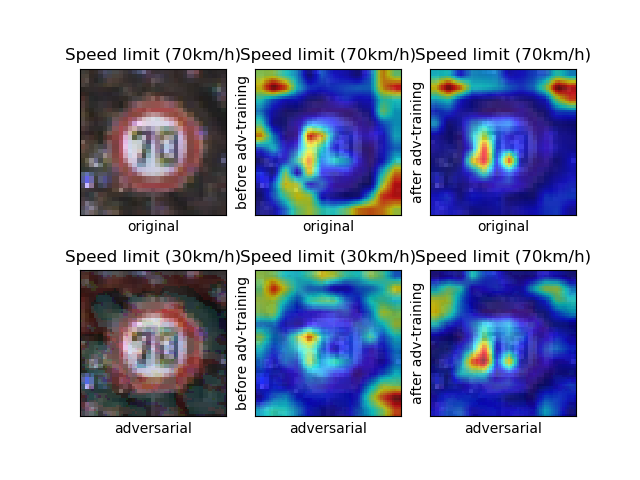
\includegraphics[scale=0.5]{graphics/Results/3.png}
    \caption{First result, first training run of alexnet using FGSM-adversarials}
    \label{fig:results} % \label has to be placed AFTER \caption (or \subcaption) to produce correct cross-references.
\end{figure}

Figure \ref{fig:results} depicts an example of results produced by the current implementation of the experiment. In this example, an alexnet was trained and fooled using FGSM. The original input (top left) is correctly classified (70km/h), the adversary input below gets misclassified (30km/h). The heatmaps in the middle show, which areas of the image were most important for the classifier's decision before adversary training. The right column shows the areas of most importance for the decision after adversarial training. After adversarial training, the adversary input gets classified correctly, and the heated area at the bottom right corner of the image disappeared. This could be interpreted as shift of "attention" to areas that seem more important and reliable for classification.

\chapter{Outline of planned calculations}

Currently, the experiment could only be done for the lenet-5 and the alexnet, using FGSM, as generating adversarial inputs for deeper architectures requires more computational power. Also, the results presented before only used one run of training and adversarial training, I expect clearer results after 10-100 iterations.
The planned calculations include training lenet-5, alexnet, vgg19 and resnet50, and generating adversarial training data for them using at least FGSM and one stronger method like deepfool. For a better resolution of the heatmaps, an upscale of the input images to at least 224x224 might be necessary, resulting in an increase of the computational costs for the whole experiment.

% Remove following line for the final thesis.
%% intro.tex
%% Copyright (C) 2014-2016 by Thomas Auzinger <thomas@auzinger.name>
%
% This work may be distributed and/or modified under the
% conditions of the LaTeX Project Public License, either version 1.3
% of this license or (at your option) any later version.
% The latest version of this license is in
%   http://www.latex-project.org/lppl.txt
% and version 1.3 or later is part of all distributions of LaTeX
% version 2005/12/01 or later.
%
% This work has the LPPL maintenance status `maintained'.
%
% The Current Maintainer of this work is Thomas Auzinger.
%
% This work consists of the files vutinfth.dtx and vutinfth.ins
% and the derived file vutinfth.cls.
% This work also consists of the file intro.tex.


\newacronym{ctan}{CTAN}{Comprehensive TeX Archive Network}
\newacronym{faq}{FAQ}{Frequently Asked Questions}
\newacronym{pdf}{PDF}{Portable Document Format}
\newacronym{svn}{SVN}{Subversion}
\newacronym{wysiwyg}{WYSIWYG}{What You See Is What You Get}

\newglossaryentry{texteditor}
{
  name={editor},
  description={A text editor is a type of program used for editing plain text files.}
}

\chapter{Introduction to \LaTeX}

Since \LaTeX\ is widely used in academia and industry, there exists a plethora of freely accessible introductions to the language.
Reading through the guide at \url{https://en.wikibooks.org/wiki/LaTeX} serves as a comprehensive overview for most of the functionality and is highly recommended before starting with a thesis in \LaTeX.

\section{Installation}

A full \LaTeX\ distribution\index{distribution} consists of not only of the binaries that convert the source files to the typeset documents, but also of a wide range of packages and their documentation.
Depending on the operating system, different implementations are available as shown in Table~\ref{tab:distrib}.
\textbf{Due to the large amount of packages that are in everyday use and due to their high interdependence, it is paramount to keep the installed distribution\index{distribution} up to date.}
Otherwise, obscure errors and tedious debugging ensue.

\begin{table}
  \centering
  \begin{tabular}{cccc}
    \toprule
    Distribution & Unix         & Windows      & MacOS        \\
    \midrule
    TeX Live     & \textbf{yes} & yes          & (yes)        \\
    MacTeX       & no           & no           & \textbf{yes} \\
    MikTeX       & no           & \textbf{yes} & no           \\
    \bottomrule
  \end{tabular}
  \caption{\TeX/\LaTeX\ distributions for different operating systems. Recomended choice in \textbf{bold}.}
  \label{tab:distrib} % \label has to be placed AFTER \caption to produce correct cross-references.
\end{table}

\section{Editors}

A multitude of \TeX\ \glspl{texteditor} are available differing in their editing models, their supported operating systems and their feature sets.
A comprehensive overview of \glspl{texteditor} can be found at the Wikipedia page  \url{https://en.wikipedia.org/wiki/Comparison_of_TeX_editors}.
TeXstudio (\url{http://texstudio.sourceforge.net/}) is recommended.

\section{Compilation}

Modern editors usually provide the compilation programs to generate \gls{pdf} documents and for most \LaTeX\ source files, this is sufficient.
More advanced \LaTeX\ functionality, such as glossaries and bibliographies, needs additional compilation steps, however.
It is also possible that errors in the compilation process invalidate intermediate files and force subsequent compilation runs to fail.
It is advisable to delete intermediate files (\verb|.aux|, \verb|.bbl|, etc.), if errors occur and persist.
All files that are not generated by the user are automatically regenerated.
To compile the current document, the steps as shown in Table~\ref{tab:compile} have to be taken.


\begin{table}
  \centering
  \begin{tabular}{rl}
    \toprule
    & Description \\
    \midrule
    1 & Scan for refs, toc/lof/lot/loa items and cites \\
    2 & Build the bibliography     \\
    3 & Link refs and build the toc/lof/lot/loa \\
    4 & Link the bibliography \\
    5 & Build the glossary \\
    6 & Build the acronyms \\
    7 & Build the index \\
    8 & Link the glossary, acronyms, and the index \\
    9 & Link the bookmarks \\
    \midrule
    & Command \\
    \midrule
    1 & \verb|pdflatex.exe  example| \\
    2 & \verb|bibtex.exe    example| \\
    3 & \verb|pdflatex.exe  example| \\
    4 & \verb|pdflatex.exe  example| \\
    5 & \verb|makeindex.exe -t example.glg -s example.ist| \\
      & \verb|              -o example.gls example.glo| \\
    6 & \verb|makeindex.exe -t example.alg -s example.ist| \\
      & \verb|              -o example.acr example.acn| \\
    7 & \verb|makeindex.exe -t example.ilg -o example.ind example.idx| \\
    8 & \verb|pdflatex.exe  example| \\
    9 & \verb|pdflatex.exe  example| \\
    \bottomrule
  \end{tabular}
  \caption{Compilation steps for this document. The following abbreviations were used: table of contents (toc), list of figures (lof), list of tables (lot), list of algorithms (loa).}
  \label{tab:compile} % \label has to be placed AFTER \caption to produce correct cross-references.
\end{table}


\section{Basic Functionality}

In this section, various examples are given of the fundamental building blocks used in a thesis.
Many \LaTeX\ commands have a rich set of options that can be supplied as optional arguments.
The documentation of each command should be consulted to get an impression of the full spectrum of its functionality.

\subsection{Floats}

Two main categories of page elements can be differentiated in the usual \LaTeX\ workflow: \textit{(i)} the main stream of text and \textit{(ii)} floating containers that are positioned at convenient positions throughout the document.
In most cases, tables, plots, and images are put into such containers since they are usually positioned at the top or bottom of pages.
These are realized by the two environments \verb|figure| and \verb|table|, which also provide functionality for cross-referencing (see Table~\ref{tab:intro} and Figure~\ref{fig:intro}) and the generation of corresponding entries in the list of figures and the list of tables.
Note that these environments solely act as containers and can be assigned arbitrary content.

\subsection{Tables}

A table in \LaTeX\ is created by using a \verb|tabular| environment or any of its extensions, e.g., \verb|tabularx|.
The commands \verb|\multirow| and \verb|\multicolumn| allow table elements to span multiple rows and columns.

\begin{table}[h] % placement specifier
  \centering
  \begin{tabular}{lll}
    \toprule
    \multicolumn{2}{c}{Position} \\
    \cmidrule{1-2} % partial horizontal rule
    Group & Abbrev & Name \\
    \midrule
    Goalkeeper & GK & Paul Robinson \\
    \midrule
    \multirow{4}{*}{Defenders} & LB & Lucus Radebe \\
                               & DC & Michael Duburry \\
                               & DC & Dominic Matteo \\
                               & RB & Didier Domi \\
    \midrule
    \multirow{3}{*}{Midfielders} & MC & David Batty \\
                                 & MC & Eirik Bakke \\
                                 & MC & Jody Morris \\
    \midrule
    Forward & FW & Jamie McMaster \\
    \midrule
    \multirow{2}{*}{Strikers} & ST & Alan Smith \\
                              & ST & Mark Viduka \\
    \bottomrule
  \end{tabular}
  \caption{Adapted example from \url{https://en.wikibooks.org/wiki/LaTeX/Tables}. This example uses rules specific to the \texttt{booktabs} package and employs the multi-row functionality of the \texttt{multirow} package.}
  \label{tab:intro} % \label has to be placed AFTER \caption to produce correct cross-references.
\end{table}

\subsection{Images}

An image is added to a document via the \verb|\includegraphics| command as shown in Figure~\ref{fig:intro}.
The \verb|\subcaption| command can be used to reference subfigures, such as Figure~\ref{fig:intro:full width} and~\ref{fig:intro:half width}.

\begin{figure}[h]
  \begin{subfigure}[b]{0.5\columnwidth}
    \centering
    
\includegraphics[width=\textwidth]{TU_INF_Logo_gray}
    \subcaption{The header logo at text width.}
    \label{fig:intro:full width}
  \end{subfigure}
  \begin{subfigure}[b]{0.5\columnwidth}
    \centering
    
\includegraphics[width=0.5\textwidth]{TU_INF_Logo_gray}
    \subcaption{The header logo at half the text width.}
    \label{fig:intro:half width}
  \end{subfigure}
  \caption{The header logo at different sizes.}
  \label{fig:intro} % \label has to be placed AFTER \caption (or \subcaption) to produce correct cross-references.
\end{figure}

\subsection{Mathematical Expressions}

One of the original motivation to create the \TeX\ system was the need for mathematical typesetting.
To this day, \LaTeX\ is the preferred system to write math-heavy documents and a wide variety of functions aids the author in this task.
A mathematical expression can be inserted inline as $\sum_{n=1}^{\infty} \frac{1}{n^2} = \frac{\pi^2}{6}$ outside of the text stream as \[ \sum_{n=1}^{\infty} \frac{1}{n^2} = \frac{\pi^2}{6} \] or as numbered equation with
\begin{equation}
\sum_{n=1}^{\infty} \frac{1}{n^2} = \frac{\pi^2}{6}.
\end{equation}

\subsection{Pseudo Code}

The presentation of algorithms can be achieved with various packages, such as \verb|algorithmic|, \verb|algorithm2e|, \verb|algorithmicx|, or \verb|algpseudocode|.
See \url{https://tex.stackexchange.com/questions/229355} for an overview.
An example of the use of the \verb|alogrithm2e| package is given with Algorithm~\ref{alg:gauss-seidel}.

\begin{algorithm}
  \SetKw{BreakFor}{break for}
  \KwIn{A scalar~$\epsilon$, a matrix $\mathbf{A} = (a_{ij})$, a vector $\vec{b}$, and an initial vector $\vec{x}^{(0)}$}
  \KwOut{$\vec{x}^{(n)}$ with $\mathbf{A} \vec{x}^{(n)} \approx \vec{b}$}
  \For{$k\leftarrow 1$ \KwTo maximum iterations}
  {
     \For{$i\leftarrow 1$ \KwTo $n$}
     {
        $x_i^{(k)} = \frac{1}{a_{ii}} \left(b_i-\sum_{j<i} a_{ij} x_j^{(k)} - \sum_{j>i} a_{ij} x_j^{(k-1)} \right)$\;
     }
     \If{$\lvert\vec{x}^{(k)}-\vec{x}^{(k-1)}\rvert < \epsilon$}
     {\BreakFor\;}
  }
  \Return{$\vec{x}^{(k)}$\;}
  \caption{Gauss-Seidel}
  \label{alg:gauss-seidel} % \label has to be placed AFTER \caption to produce correct cross-references.
\end{algorithm}

\section{Bibliography}

The referencing of prior work is a fundamental requirement of academic writing and well supported by \LaTeX.
The \textsc{Bib}\TeX\ reference management software is the most commonly used system for this purpose.
Using the \verb|\cite| command, it is possible to reference entries in a \verb|.bib| file out of the text stream, e.g., as~\cite{Turing1936}.
The generation of the formatted bibliography needs a separate execution of \verb|bibtex.exe| (see Table~\ref{tab:compile}).

\section{Table of Contents}

The table of contents is automatically built by successive runs of the compilation, e.g., of \verb|pdflatex.exe|.
The command \verb|\setsecnumdepth| allows the specification of the depth of the table of contents and additional entries can be added via \verb|\addcontentsline|.
The starred versions of the sectioning commands, i.e., \verb|\chapter*|, \verb|\section*|, etc., remove the corresponding entry from the table of contents.

\section{Acronyms / Glossary / Index}

The list of acronyms, the glossary, and the index need to be built with a separate execution of \verb|makeindex| (see Table~\ref{tab:compile}).
Acronyms have to be specified with \verb|\newacronym| while glossary entries use \verb|\newglossaryentry|.
Both are then used in the document content with one of the variants of \verb|\gls|, such as \verb|\Gls|, \verb|\glspl|, or \verb|\Glspl|.
Index items are simply generated by placing \verb|\index|\marg{entry} next to all the words that correspond to the index entry \meta{entry}.
Note that many enhancements exist for these functionalities and the documentation of the \verb|makeindex| and the \verb|glossaries| packages should be consulted.

\section{Tips}

Since \TeX\ and its successors do not employ a \gls{wysiwyg} editing scheme, several guidelines improve the readability of the source content:
\begin{itemize}
\item Each sentence in the source text should start with a new line.
      This helps not only the user navigation through the text, but also enables revision control systems (e.g. \gls{svn}, Git) to show the exact changes authored by different users.
      Paragraphs are separated by one (or more) empty lines.
\item Environments, which are defined by a matching pair of \verb|\begin{name}| and \verb|\end{name}|, can be indented by whitespace to show their hierarchical structure.
\item In most cases, the explicit use of whitespace (e.g. \verb|\hspace{4em}| or \verb|\vspace{1.5cm}|) violates typographic guidelines and rules.
      Explicit formatting should only be employed as a last resort and, most likely, better ways to achieve the desired layout can be found by a quick web search.
\item The use of bold or italic text is generally not supported by typographic considerations and the semantically meaningful \verb|\emph{|\texttt{$\dots$}\verb|}| should be used.
\end{itemize}

The predominant application of the \LaTeX\ system is the generation of \gls{pdf} files via the \textsc{Pdf}\LaTeX\ binaries.
In the current version of \textsc{Pdf}\LaTeX, it is possible that absolute file paths and user account names are embedded in the final \gls{pdf} document.
While this poses only a minor security issue for all documents, it is highly problematic for double blind reviews.
The process shown in Table~\ref{tab:ps2pdf} can be employed to strip all private information from the final \gls{pdf} document.

\begin{table}[h]
  \centering
  \begin{tabular}{rl}
  \toprule
  & Command \\
  \midrule
  1 & Rename the \gls{pdf} document \verb|final.pdf| to \verb|final.ps|. \\
  2 & Execute the following command: \\
    & \verb|ps2pdf -dPDFSETTINGS#/prepress ^| \\
    & \verb| -dCompatibilityLevel#1.4 ^| \\
    & \verb| -dAutoFilterColorImages#false ^| \\
    & \verb| -dAutoFilterGrayImages#false ^| \\
    & \verb| -dColorImageFilter#/FlateEncode ^| \\
    & \verb| -dGrayImageFilter#/FlateEncode ^| \\
    & \verb| -dMonoImageFilter#/FlateEncode ^| \\
    & \verb| -dDownsampleColorImages#false ^| \\
    & \verb| -dDownsampleGrayImages#false ^| \\
    & \verb| final.ps final.pdf| \\
  \bottomrule
  \end{tabular}

  On Unix-based systems, replace \verb|#| with \verb|=| and \verb|^| with \verb|\|.
  \caption{Anonymization of \gls{pdf} documents.}
  \label{tab:ps2pdf}
\end{table}

\section{Resources}

\subsection{Useful Links}

In the following, a listing of useful web resources is given.
\begin{description}
\item[\url{https://en.wikibooks.org/wiki/LaTeX}] An extensive wiki-based guide to \LaTeX.
\item[\url{http://www.tex.ac.uk/faq}] A (huge) set of \gls{faq} about \TeX\ and \LaTeX.
\item[\url{https://tex.stackexchange.com/}] The definitive user forum for non-trivial \LaTeX-related questions and answers.
\end{description}

\subsection[Comprehensive TeX Archive Network]{\gls{ctan}}

The \gls{ctan} is the official repository for all \TeX\ related material.
It can be accessed via \url{https://www.ctan.org/} and hosts (among other things) a huge variety of packages that provide extended functionality for \TeX\ and its successors.
Note that most packages contain \gls{pdf} documentation that can be directly accessed via \gls{ctan}.

In the following, a short, non-exhaustive list of relevant \gls{ctan}-hosted packages is given together with their relative path.
\begin{description}[itemsep=0ex]
\item[\href{https://www.ctan.org/pkg/algorithm2e}{algorithm2e}] Functionality for writing pseudo code.
\item[\href{https://www.ctan.org/pkg/amsmath}{amsmath}] Enhanced functionality for typesetting mathematical expressions.
\item[\href{https://www.ctan.org/pkg/amsfonts}{amssymb}] Provides a multitude of mathematical symbols.
\item[\href{https://www.ctan.org/pkg/booktabs}{booktabs}] Improved typesetting of tables.
\item[\href{https://www.ctan.org/pkg/enumitem}{enumitem}] User control over the layout of lists (\verb|itemize|, \verb|enumerate|, \verb|description|).
\item[\href{https://www.ctan.org/pkg/fontenc}{fontenc}] Determines font encoding of the output.
\item[\href{https://www.ctan.org/pkg/glossaries}{glossaries}] Create glossaries and list of acronyms.
\item[\href{https://www.ctan.org/pkg/graphicx}{graphicx}] Insert images into the document.
\item[\href{https://www.ctan.org/pkg/inputenc}{inputenc}] Determines encoding of the input.
\item[\href{https://www.ctan.org/pkg/l2tabu}{l2tabu}] A description of bad practices when using \LaTeX.
\item[\href{https://www.ctan.org/pkg/mathtools}{mathtools}] Further extension of mathematical typesetting.
\item[\href{https://www.ctan.org/pkg/memoir}{memoir}] The document class on upon which the \verb|vutinfth| document class is based.
\item[\href{https://www.ctan.org/pkg/multirow}{multirow}] Allows table elements to span several rows.
\item[\href{https://www.ctan.org/pkg/pgfplots}{pgfplots}] Function plot drawings.
\item[\href{https://www.ctan.org/pkg/pgf}{pgf/TikZ}] Creating graphics inside \LaTeX\ documents.
\item[\href{https://www.ctan.org/pkg/subcaption}{subcaption}] Allows the use of subfigures and enables their referencing.
\item[\href{https://www.ctan.org/tex-archive/info/symbols/comprehensive/}{symbols/comprehensive}] A listing of around 5000 symbols that can be used with \LaTeX.
\item[\href{https://www.ctan.org/pkg/voss-mathmode}{voss-mathmode}] A comprehensive overview of typesetting mathematics in \LaTeX.
\item[\href{https://www.ctan.org/pkg/xcolor}{xcolor}] Allows the definition and use of colors.
\end{description} % A short introduction to LaTeX.

\backmatter

% Use an optional list of figures.
\listoffigures % Starred version, i.e., \listoffigures*, removes the toc entry.

% Use an optional list of tables.
\listoftables % Starred version, i.e., \listoftables*, removes the toc entry.

% Use an optional list of alogrithms.
\listofalgorithms
\addcontentsline{toc}{chapter}{List of Algorithms}

% Add an index.
\printindex

% Add a glossary.
\printglossaries

% Add a bibliography.
\bibliographystyle{alpha}
\bibliography{intro}

\end{document}